\documentclass[times, utf8, seminar, numeric]{fer}
\usepackage[utf8]{inputenc}
\usepackage[T1]{fontenc}
\usepackage{currvita}
\usepackage{graphicx}
\usepackage{epstopdf}
\usepackage{listings}
\usepackage{textcomp}
\usepackage{booktabs}
\usepackage{algorithmic}
\usepackage{algorithm}


% definicija jezika koji nema nista, pa se nista ne naglasava
% koristi se za troadresni kod, ispise tokena i slicno
\lstdefinelanguage{blank}{
	sensitive=false, 
	morecomment=[l]{;},
}

% koristimo zadebljane vektore, a ne strelice
\renewcommand{\vec}[1]{\mathbf{#1}}

% neke boje koje koristimo u formatiranju ispisa
\usepackage{color}
\definecolor{mygreen}{rgb}{0,0.6,0}
\definecolor{mylightgray}{rgb}{0.95,0.95,0.95}

% definicija formatiranja ispisa, ponesto promjenjena u odnosu na pretpostavljenu
\lstset{ %
  backgroundcolor=\color{mylightgray},   % choose the background color; you must add \usepackage{color} or \usepackage{xcolor}
  basicstyle=\footnotesize\ttfamily,        % the size of the fonts that are used for the code
  breakatwhitespace=false,         % sets if automatic breaks should only happen at whitespace
  breaklines=true,                 % sets automatic line breaking
  captionpos=b,                    % sets the caption-position to bottom
  commentstyle=\color{mygreen},    % comment style
  deletekeywords={...},            % if you want to delete keywords from the given language
  escapeinside={\%*}{*)},          % if you want to add LaTeX within your code
  extendedchars=true,              % lets you use non-ASCII characters; for 8-bits encodings only, does not work with UTF-8
  frame=none,                    % adds a frame around the code
  keepspaces=true,                 % keeps spaces in text, useful for keeping indentation of code (possibly needs columns=flexible)
  keywordstyle=\color{blue},       % keyword style
  language=c,           	       % the language of the code
  morekeywords={*,...},            % if you want to add more keywords to the set
  numbers=none,                    % where to put the line-numbers; possible values are (none, left, right)
  numbersep=5pt,                   % how far the line-numbers are from the code
  numberstyle=\tiny\color{gray}, % the style that is used for the line-numbers
  rulecolor=\color{black},         % if not set, the frame-color may be changed on line-breaks within not-black text (e.g. comments (green here))
  showspaces=false,                % show spaces everywhere adding particular underscores; it overrides 'showstringspaces'
  showstringspaces=false,          % underline spaces within strings only
  showtabs=false,                  % show tabs within strings adding particular underscores
  stepnumber=2,                    % the step between two line-numbers. If it's 1, each line will be numbered
  stringstyle=\color{red},     % string literal style
  tabsize=2,                       % sets default tabsize to 2 spaces
  title=\lstname                   % show the filename of files included with \lstinputlisting; also try caption instead of title
}

\title{Detekcija lica u grupnim scenama}

\author{T. Antunović, S. Čolaković, E. Smoljan, F. Stamenković, I. Weber}

\voditelj{Marijo Maračić}


\begin{document}

\maketitle

\tableofcontents

\chapter{Uvod i problematika}

\section{Detekcija lica}

Detekcija lica je prvi korak u sustavima za raspoznavanje lica u proizvoljnim scenama. Cilj detekcije je lokalizacija i ekstrakcija lica iz pozadine. Ljudsko lice ima visok stupanj varijabilnosti na slikama, što čini detekciju lica teškim problemom u području računalnog vida. Ovaj problem je detaljno istraživan i postoje različiti načini kako dobiti zadovoljavajuće rezultate.

\section{Prepoznavanje lica}

Prepoznavanje lica je zadatak pridodavanja oznake slici lica, pri čemu je oznaka uglavnom identifikator osobe. U tu svrhu potreban je inicijalni skup poznatih lica (slika identificiranih lica) i algoritam prepoznavanja. Primjene sustava prepoznavanja lica u sigurnosti i komercijalnim/korisničkim područjima su brojne, te se ovo područje aktivno istražuje. Rastom računalne snage, padom cijena senzora (kamera) te razvojem sve snažnijih algoritama prepoznavanja kvaliteta raspoznavanja je došla do točke praktične primjenjivosti.

\chapter{Pregled postojećih rješenja}

\section{Detekcija lica}

Sustavi za detekciju lica se mogu podijeliti na sustave temeljene na značajkama \engl{feature-based} i sustave temeljene na slici \engl{image-based} \cite{CVIU2001:Hjelmas}. Oni koji su temeljeni na značajkama mogu vršiti analizu slike niskog nivoa koja se oslanja na detekciju rubova, područja intenziteta ili boje, mogu vršiti analizu značajki ili kreirati modele aktivnih oblika \engl{active shape models}. Sustavi temeljeni na slici se dijele na tri glavne skupine: neuronske mreže, metode linearnih potprostora te razne statističke pristupe.

\subsection{Detekcija bazirana na značajkama}

Sustav za robusnu detekciju lica u realnom vremenu opisan u \cite{Viola04robustreal-time} može poslužiti kao primjer sustava baziranom na značajkama. Temelji se na prikazu slike koji su nazvali “integralna slika”, jednostavnom klasifikatoru koji koristi AdaBoost algoritam učenja za izbor najbitnijih značajki iz velikog skupa, te na kaskadnom kombiniranju klasifikatora koje omogućuje da pozadinske regije budu brzo odbačene i da što je moguće veći dio računanja koncentrira na regije koje imaju veću vjerojatnost da predstavljaju lice.

\subsubsection{Modeli aktivnih oblika}

Modeli aktivnih oblika predstavljaju značajke višeg nivoa od prethodno spomenutih modela. Kada se inicijalizira u blizini značajke model aktivnog oblika će kroz interakciju s lokalnim značajkama poput rubova i osvjetljenosti postepeno zauzeti oblik značajke višeg nivoa. Na taj način se mogu koristiti ne samo za detekciju lica nego i za prepoznavanje lica kroz označavanje bitnih regija poput očiju, obrva, usta i nosa \cite{prabhu_utsav_facialrecog}.

\subsubsection{Detekcija temeljena na boji}

Postupak detekcije lica temeljene na boji kojeg koriste radovi poput \cite{Senior:2002:FDC:513073.513082} i \cite{conf/isda/ChandrappaR12} je sljedeći. Prvo detektirati područja na slici koja odgovaraju koži na temelju boje slikovnih elemenata. Potom pronađena područja klasificirati kao lica ili ne-lica.  Klasifikacija je potrebna zato što se segmentacijom po boji izdvajaju i dijelovi slike koji prikazuju ostale dijelove tijela (primjerice ruke). U radu \cite{Senior:2002:FDC:513073.513082} se klasifikaciji pristupa tako da se najprije odrede područja u kandidatima za lice koji odgovaraju očima i ustima te se lice prihvaća ako je ocjena pronađenih kandidata bolja od neke granične vrijednosti. 

\begin{figure}[!htb]
\centering
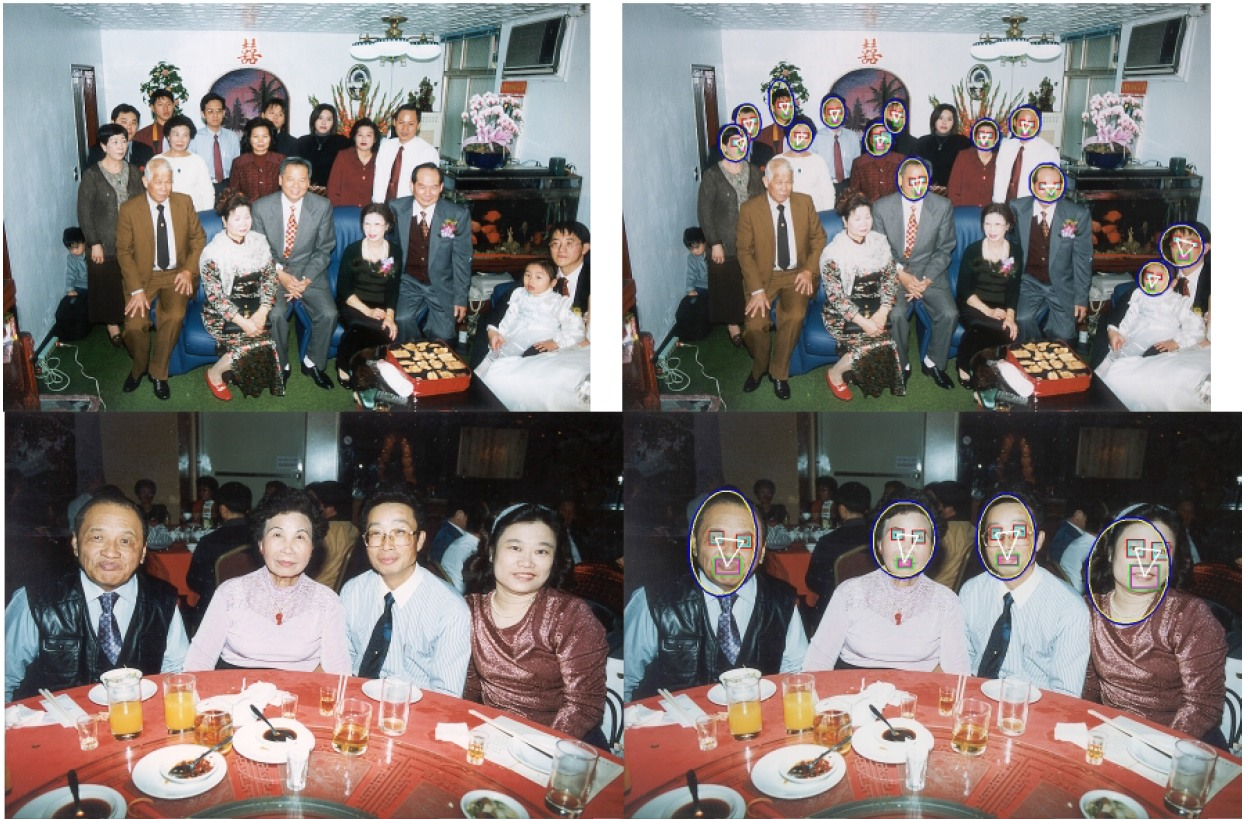
\includegraphics[width=\textwidth]{raw/detekcija_pr1.jpg}
\caption{Primjer detekcije lica u radu \cite{Senior:2002:FDC:513073.513082}.}
\label{fig:detekcija_pr1}
\end{figure}

Rad \cite{conf/isda/ChandrappaR12} klasifikaciji pristupa tako da na temelju postojećeg skupa slika lica stvara sliku prosječnog lica. Klasifikacija se vrši tako da se računa korelacija kandidata sa prosječnim licem. Ovaj pristup detaljnije je opisan u poglavlju \ref{sec:predlozeno_detekcija}.

\subsection{Detekcija bazirana na slici}

\subsubsection{Neuronske mreže}

Pri detekciji lica korištenjem neuronskih mreža u \cite{Rowley98neuralnetwork-based} korišteno je više mreža koje su obavljale različite zadatke. Prva neuronska mreža je vršila procjenu poze potencijalnih regija koje predstavljaju lice. Nakon nje se vršilo pretprocesiranje s ciljem smanjivanja varijacija uzrokovanih osvjetljenjem i razlikama vezanim za kamere. Nakon toga za svaku pozu je korišteno nekoliko neuronskih mreža koje su učile različite stvari iz podataka za treniranje i davale različite rezultate. U posljednjem sloju njihovi izlazi su kombinirani koristeći jednostavnu heuristiku s ciljem povećanja točnih detekcija.

Pristup zasnovan na dubokim konvolucijskim neuronskim mrežama \cite{zhang2014improving} na efikasan način izvlači značajke tokom učenja i na FDDB bazi trenutno ostvaruje najbolje rezultate. 

\subsubsection{Metode linearnih podprostora}

Metode linearnih potprostora su metode poput PCA \engl{principal component analysis}, ICA \engl{independent component analysis}, LDA \engl{linear discriminant analysis} i FA \engl{factor analysis}. Pošto unutar predloženog rješenja (poglavlje \ref{sec:predlozeno}) koristimo PCA i ICA algoritme, ovdje ih nećemo dublje razrađivati.

\subsubsection{Statistički pristupi}

Kao primjer statističkog pristupa u detekciji lica može poslužiti FloatBoost učenje bazirano na AdaBoost algoritmu \cite{Li04floatboostlearning}. FloatBoost nakon svake iteracije AdaBoost učenja koristi povratni mehanizam za direktnu minimizaciju pogreške. Postiže manju pogrešku učenja i generalizacije koristeći manji broj slabih klasifikatora od AdaBoost algoritma.

\section{Raspoznavanje lica}

Većina algoritama za prepoznavanje lica koriste neki oblik preprocesiranja slike kako bi se dobile značajke pogodne za klasifikaciju. U radu koji nam je dan kao glavna osnova za izradu projekta se koriste metode PCA (principle component analysis) i ICA (independent component analysis), detaljno opisane i uspoređene u \cite{Draper:2003:RFP:950135.950141}. U literaturi ne postoji konceznus o tome koja je metoda bolja u kojim situacijama, ali rad dolazi do zaključka da implementacije ICA metode u prosjeku daju bolje performanse i višu preciznost.

Rad \cite{5539992} prezentira algoritam raspoznavanja lica u kojem autori nastoje omogućiti precizno raspoznavanje bez obzira na smetnje poput prekrivanja lica, proizvoljnosti položaja i vizualnog šuma. Koriste naučeni koder kako bi dobili opisnik koji se pred kraj obrađuje PCA (principle component analysis) metodom kako bi se smanjile njegove dimenzije i poboljšale performanse algoritma.   Detaljnije, nakon detektiranja lica pronalaze se komponente lica poput nosa, očiju i obraza te se nakon filtriranja šuma dobivaju digitalne reprezentacije njihovih značajki u obliku vektora. Vektori se normaliziraju te se pomoću njih utvrđuje da li se radi o traženom licu. Pretpostavlja se, naravno, da je koder naučen na značajkama lica koja su korištena u treniranju. Algoritam je također u stanju paralelno računanju značajka lica odrediti položaj lica te tu informaciju iskoristiti u konačnoj odluci, čime se poboljšava preciznost. Možda najzanimljiviji dio algoritma je mogućnost kombiniranja više opisnika koristeći poptorni vektor, čime algoritam u konačnosti postiže preciznost od visokih 84.45\% na LFW \cite{Huang_labeledfaces} bazi slika.

Rad \cite{Lu_imageanalysis} daje pregled smjera u kojem se trenutno kreću sustavi za rapoznavanje lica i algoritmi koji se pri tome koriste. Opisuje nagli porast interesa za dotično područje u proteklim godinama zbog napretka na području strojnog učenja i računalne grafike te potražnje za sustavima koji koriste tehnologije kojima se bavi računalni put, a neka od primjena su prepoznavanje profilnih slika, automatsko praćenje i promatranje većeg broja ljudi, digitalna rekonstrukcija lica itd. Autor dijeli algoritme za prepoznavanje lica u dvije velike skupine. Prva skupina su algoritmi koji se osnivaju na izgledu, odnosno slikama pojedinaca te se obično koriste u paru sa vektorskim prikazom slika koje obrađuju, što znači da u ovu skupinu pripadaju prije navedeni radovi, a na internetu se nude razne baze podataka slika poput \textit{AT\&T Cambridge} \footnote{http://www.cl.cam.ac.uk/research/dtg/attarchive/facedatabase.html}. Sa druge strane su algoritmi bazirani na modelu, koji nastoje promatrati lica kao 3D modele koji vjerodostojno prikazuju lice sa svim njegovim značajkama te pomoću toga vrše prepoznavanje. Autor navodi neke od algoritama obje skupine te opisuje prednosti i mane svake skupine.

\section{Primjer primjene: Bostonski maraton}

Zanimljiv primjer korištenja računalnog vida u svrhu detekcije i raspoznavanja lica je analiza bombaškog napada na Bostonski maraton 2013. godine.

Detekcija lica na slikama maratona se raspravlja u radu \cite{barr2014effectiveness}, gdje se predlaže algoritam baziran na Viola-Jones algoritmu \cite{Viola01rapidobject}. Koristeći integralnu sliku i pomični prozor, algoritam prolazi kroz cijelu sliku te provjerava za svaki njen dio da li se na njemu nalazi neko lice. S obzirom da na značajke lica uvelike utječe njegova nakrenutost, algoritam je opremljen detekcijom lica okrenutih prema naprijed, ulijevo ili udesno. Detekcija se vrši nad pomičnim prozorm za svaku od navedenih orjentacija. Algoritam je, osim na slikama maratona,  testiran i na FDDB ispitnom skupu te je dao bolje rezultate od ostalih rješenja. Nažalost, algoritam se pokazao osjetljivim na utjecaj vizualnog šuma i prekrivanja lica, a problem pozicije lica nije u potpunosti riješen.

Raspoznavanje lica je također provedeno nad slikama Bostonskog maratona, a time se bavi rad \cite{Klontz13acase}, koji testira dva komercijalna sustava za raspoznavanje lica, PittPatt 5.2.2 i NeoFace 3.1 nad slikama nekooperativnih osumnjičenika, zbog čega su same slike slabije kvalitete. Valja napomenuti da je istraga vezana uz maraton mogla biti puno kraća uz valjane algoritme raspoznavanja, budući da su se slike lica braće Tsarnaev, glavnih osumnjičenika, nalazile u službenoj bazi podataka. Iako ne nudi uvid u rad samih sustava, rad prikazuje varijacije u dobivenim rezultatima ovisno o načinu izbora skupa sa kojim se lica uspoređuju. Sustavi su prvo testirani nad cijelom bazom podataka koja se sastoji od milijun profila te su za svaku danu sliku dobivene tri osobe koje najviše odgovaraju traženom licu, pri čemu je samo NeoFace uspio ispravno prepoznati jednu sliku mlađeg brata. Nakon toga su za svakog brata uneseni dodatni podaci poput spola, rase i dobi što je smanjilo broj mogućih osoba za otprilike šest puta u oba slučaja, a povećanje kvalitete je bilo proporcionalno tom smanjenju. Na kraju se isprobala varijanta sa spajanjem rezultata za svaku osobu koju se pokušalo prepoznati u bazi, čime se dobivaju bolji rezultati ako su pojedinačne slike davale slične rezultate, ali gori ukoliko nisu. Sve u svemu, rad dobro pokazuje utjecaj pristupa testnom skupu. 

\chapter{Predložena implementacija}
\label{sec:predlozeno}

U radu koji će poslužiti kao osnova za izradu ovog projekta \cite{conf/isda/ChandrappaR12} za detekciju lica se vrši jednostavna analiza niskog nivoa temeljena na segmentaciji boja, slike i višeslojnom filtriranju tako dobivenih regija koristeći različite vrijednosti pragova sličnosti s prosječnim licem. Klasifikacija lica temelji se na PCA i LCA algoritmima opisanim u nastavku. Dijagram sustava prikazan je na slici \ref{fig:diagram}

\begin{figure}[!htb]
\centering
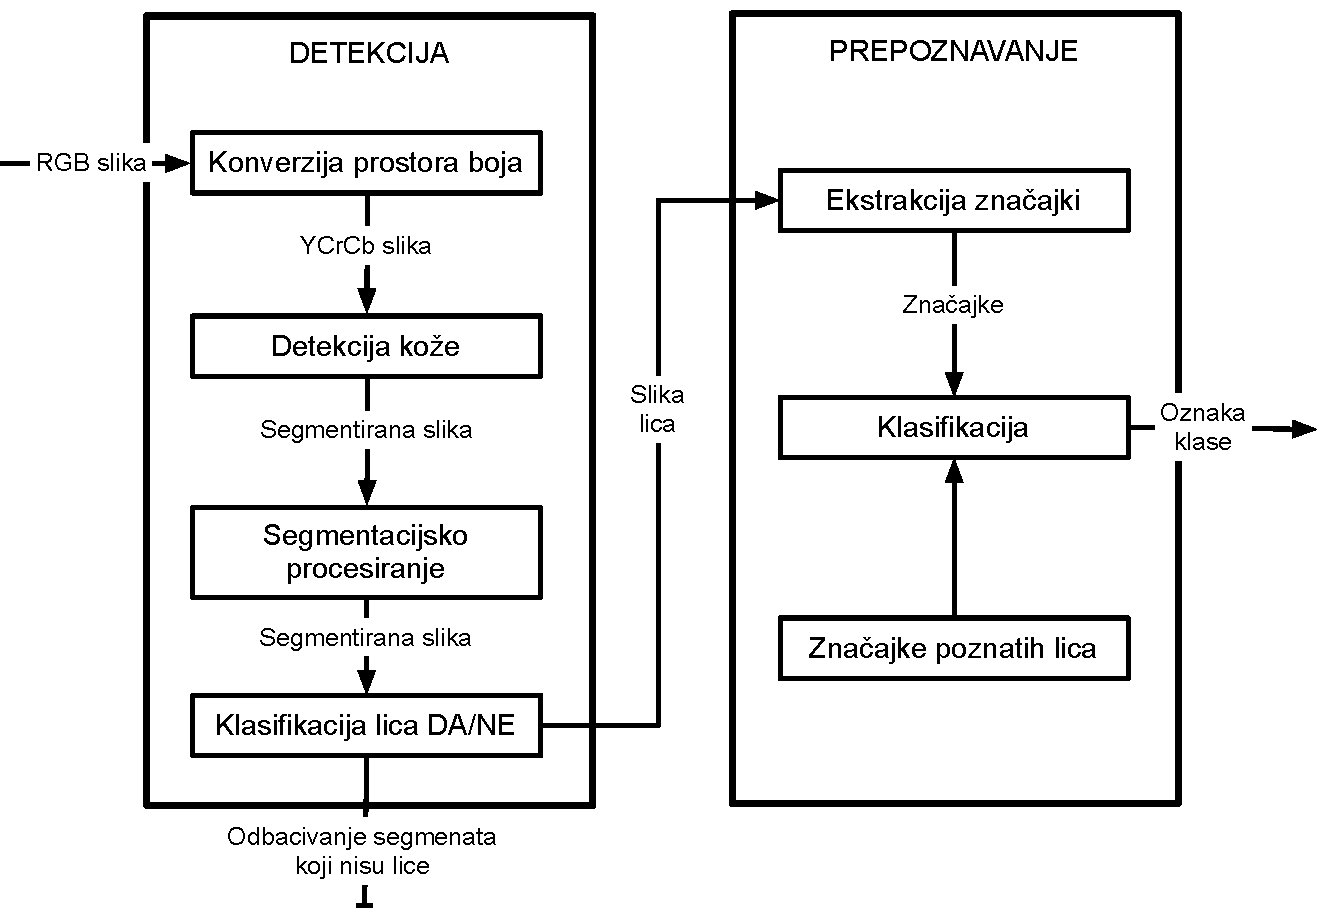
\includegraphics[width=\textwidth]{raw/Diagram.pdf}
\caption{Dijagram sustava, protok podataka.}
\label{fig:diagram}
\end{figure}

\section{Detekcija lica}
\label{sec:predlozeno_detekcija}

Razmotrimo implementaciju detekcije lica temeljene na boji opisanu u \cite{Senior:2002:FDC:513073.513082} i \cite{conf/isda/ChandrappaR12}. Prvi dio postupka obuhvaća pronalazak slikovnih elemenata boje kože. Kako bi se bavio efikasno, sliku je potrebno iz RGB prostora konvertirati u YCrCb ili YIQ prostor i onda izgraditi binarnu sliku (masku) u kojoj je svaki piksel označen ako komponente piksela zadovoljavaju uvjet pripadanja koži. Sam uvjet pripadanja piksela području kože varira kroz radove: u \cite{rahman_face_det_gender_svm} koji za obradu koristi YCrCb prikaz uvjet glasi 90<Y<180, 90<Cr<130, 80<Cb<150, dok je u radu \cite{Senior:2002:FDC:513073.513082} utvrđena i opisana zavisnost između Cr, Cb i Y komponenti te se prvo izvršava nelinearna transformacija Cr i Cb komponenti i nakon toga ispituje uvjet pripadanja. Ove opisane metode su empirijske i moguće je da svaki istraživački tim definira svoje u sklopu svog rada. U radu \cite{Senior:2002:FDC:513073.513082} se prije samog stvaranja binarne slike početna slika još provlači kroz fazu pretprocesiranja u kojoj se gleda umanjiti utjecaj izvora svijetlosti na boje u slici. Dobivena binarna maska se  još dodatno može transformirati operacijama otvaranja, filtriranja, dilatacije, erozije i zatvaranja kako bi se postigle kompaktnije maske koje predstavljaju moguća područja lica. Dobivena područja se iz slike izvlače postupcima segmentacije.

\begin{figure}[!htb]
\centering
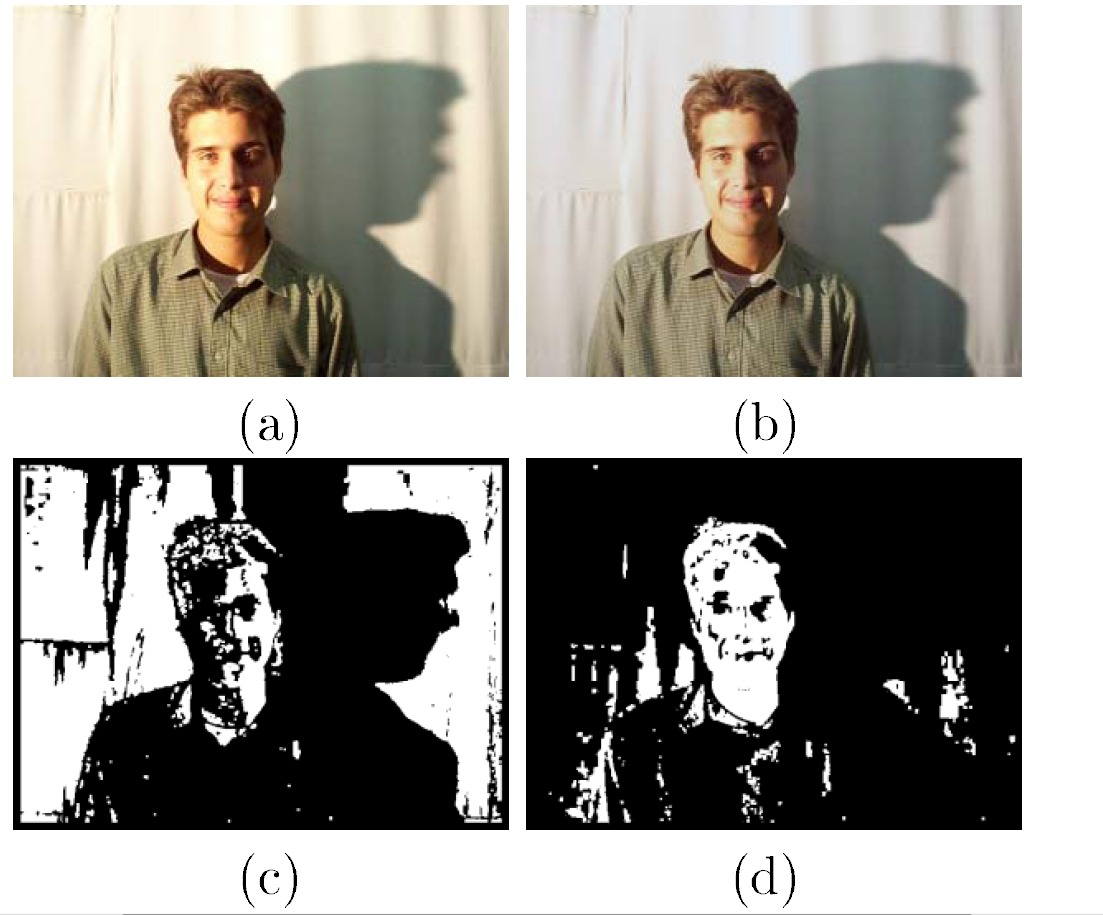
\includegraphics[width=\textwidth]{raw/skin_det.jpg}
\caption{Određivanje područja na slici koja pripadaju koži uz normalni i smanjeni utjecaj svijetlosti.}
\label{fig:skin_det}
\end{figure}

Potom je potrebno područja slike dobivena segmentacijom klasificirati kao lica odnosno ne-lica. U skladu sa \cite{conf/isda/ChandrappaR12} klasifikacija se obavlja na sljedeći način. Na samom početku postoji skup lica koja čine skup za učenje, od tih se lica stvara slika prosječnog lica i za svakog kandidata lica se računa korelacija kandidata sa prosječnim licem. Ako je ta korelacija niska kandidat se odbacuje, inače ako je područje kandidata dovoljno veliko on se prihvaća kao područje lica. Test korelacije je sličan načinu na koji se maximal rejection classifier (MRC) koristi za detekciju lica opisanog u radu \cite{Elad00patterndetection}. Prihvaćanje kandidata na temelju veličine područja se obavlja koristeći prilagođavajuću granicu prihvaćanja kako bi se omogućilo prihvaćanje malih lica na slici, a istodobno odbacivalo manja područja za koje je prolazak testa korelacije moguć (dijelovi tijela poput ruku).

\section{Prepoznavanje lica}

Nakon što su lica detektirana, izrezana i skalirana lica se prepoznaju korištenjem kombinacije PCA i ICA algoritama. Iako se PCA algoritam može koristiti samostalno za prepoznavanje lica u ovom ćemo ga radu koristiti kao korak predprocesiranja slike. Uz pomoć PCA smanjujemo dimenzionalnost vektora značajki. Ovaj pristup pridonosi kvaliteti rješenja iz više razloga, značajke sa malom varijancom su vjerojatno posljedica šuma i nepoželjne su te se smanjuje složenost modela \cite{Draper:2003:RFP:950135.950141}. Nakon toga, lica se prepoznaju ICA metodom. Postoje dvije arhitekture te više algoritama ICA metode koji se mogu primjeniti u ovome slučaju.

\subsection{ICA}

ICA (eng. Independent Component Analysis) metoda slična je PCA (eng. Principal Component Analysis) te se može smatrati njenom generalizacijom. Razlika između njih leži u tome što PCA daje nekorelirane bazične vektore, a ICA statistički neovisne vektore. ICA rješava BSS (eng. blind source separation) problem, pokušava prikazati signal kao linearnu kombinaciju nezavisnih signala.

Ako je $\vec{s}$ vektor nepoznatih nelinearnih signala, $\vec{x}$ opaženi signal i $\vec{A}$ matrica transformacije, pokušavamo riješiti sljedeću jednakost:

\[
\vec{x} = \vec{A} \vec{s}
\]

Pretpostavka je da $\vec{A}$ nema inverz. ICA algoritmi pokušavaju naći $\vec{A}$ ili $\vec{W}$ iz sljedeće jednadžbe:

\[
\vec{u} = \vec{W} \vec{x} = \vec{W} \vec{A} \vec{s}
\]

Moguće je da ne postoji matrica $\vec{W}$ koja u potpunosti zadovoljava ovu jednadžbu. $\vec{W}$ se aproksimira iterativnim postupcima koji maksimiziraju neovisnost bazičnih vektora. Ona se ne maksimizira izravno već se odabiru funkcije koje imaju maksimum kada su vektori nezavisni.
ICA algoritam InfoMax maksimizira entropiju postupkom gradijentnog spusta, dok FastICA maksimizira gdje je $G$ nekvadratna funkcija, $v$ slučajna varijabla, a $c$ neka pozitivna konstanta. Svi ICA algoritmi konvergiraju u isto rješenje te ne postoje velike razlike u njihovim performansama \cite{Draper:2003:RFP:950135.950141}.

\subsubsection{Arhitektura I}
Postoje dva načina za primjenu ICA-e na problemima prepoznavanja lica. Kod prvog načina ulazne slike lica $\vec{X}$ promatraju se kao linearna kombinacija nezavisnih slika $\vec{S}$. Primjenom InfoMax algoritma dobivamo U, aproksimaciju nezavisnih bazičnih slika. Slika \ref{fig:prepoznavanje_arh1} prikazuje opisanu arhitekturu. Ova arhitektura daje lokalizirane značajke te je bolja za prepoznavanje pokreta lica \cite{Draper:2003:RFP:950135.950141}.

\begin{figure}[!htb]
\centering
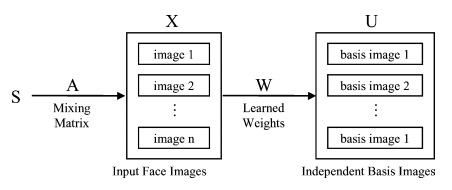
\includegraphics{raw/prepoznavanje_arh1.jpg}
\caption{Arhitektura I}
\label{fig:prepoznavanje_arh1}
\end{figure}


\subsubsection{Arhitektura II}
Za razliku od prve, druga arhitektura daje globalne značajke te postiže bolje rezultate kod prepoznavanja lica.
Cilj ovog načina ICA jest pronalazak nezavisnih koeficijenata za ulazne podatke. Matrica $\vec{X}$ predstavlja slikovne elemente (eng. pixels) slike, $\vec{S}$ nezavisne koeficijente ulazne slike, dok je $\vec{A}$ matrica bazičnih slika.

\begin{figure}[!htb]
\centering
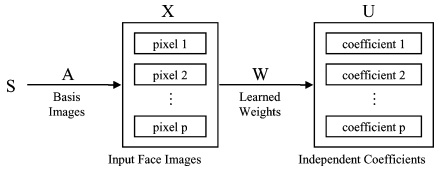
\includegraphics{raw/prepoznavanje_arh2.jpg}
\caption{Arhitektura II}
\label{fig:prepoznavanje_arh2}
\end{figure}

Na slici \ref{fig:prepoznavanje_znacajke} možemo vidjeti kakve se značajke dobiju prikazanim arhitekturama. Gornji red prikazuje PCA značajke, srednji ICA značajke uz arhitekturu I, a donji red ICA uz arhitekturu II. Jasno je vidljivo da su značajke ICA II arhitekture globalne. U radu \cite{Draper:2003:RFP:950135.950141} testirani su ICA i PCA algoritmi različitih arhitektura. Vidljivo je da ICA arhitektura II daleko najuspješnija u prepoznavanju lica, pa ćemo je koristiti i u ovom radu. ICA algoritam FastICA postiže malo bolje rezulate od InfoMax-a te njega biramo za ovaj rad.

\begin{figure}[!htb]
\centering
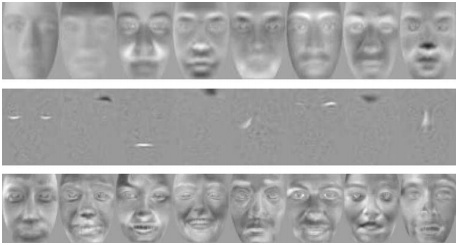
\includegraphics{raw/prepoznavanje_znacajke.jpg}
\caption{Značajke dobivene PCA, ICA arhitektura I i ICA arhitektura II}
\label{fig:prepoznavanje_znacajke}
\end{figure}

\section{Korištene baze}

Zadatak projekta je detekcija i prepoznavanje lica u proizvoljnim scenama. Implementaciju sustava potrebno
je testirati na standardiziranoj bazi podataka kako bi se rezultati mogli usporediti sa
drugim implementacijama.

U trenutku pisanja nismo pronašli bazu koja bi se mogla koristiti za oba koraka algoritma (detekciju i
prepoznavanje). Takva baza morala bi sadržavati slike proizvoljnih scena u kojima su lica označena
lokacijski (položaj lica na slici) i labelirana (identifikator osobe svakog označenog lica). Stoga
predlažemo evaluaciju cjelokupnog algoritma u dva koraka. Prvo evaluiramo detekciju lica na prikladnoj
bazi, a potom na drugoj bazi evaluiramo algoritam prepoznavanja. Iako ovaj pristup nije idealan, omogućava
evaluaciju na standardnim bazama i usporedbu sa drugim sustavima.

\subsubsection{Detekcija lica}

Postoje brojne baze u kojima je lice prikazano frontalno ili pod nekoliko različitih
kutova \footnote{http://robotics.csie.ncku.edu.tw/Databases/FaceDetect\_PoseEstimate.htm \\
http://www.face-rec.org/databases/}. Većina tih baza sadrži vrlo strukturirane fotografije. Lice najčešće
zauzima veliki dio slike, centralno je pozicionirano i prikazano u cjelokupnosti. U tom smislu one
nisu prikladnu za evaluaciju sustava za detekciju lica u proizvoljnim scenama.

Baza podataka
FDDB \footnote{http://vis-www.cs.umass.edu/fddb/} jedna je od rijetkih koje sadrže slike uistinu
prozvoljnih scena, s označenim područjima koja prikazuju lica. Sadrži 5171 lica označenih
unutar 2845 fotografije. Često se koristi te postoje
dobro dokumentirani rezultati za velik broj sustava za detekciju, opisano u 
\cite{fddbTech}. Stoga smatramo da je baza prikladna za evaluaciju našeg sustava detekcije.

\subsubsection{Prepoznavanje}

Mnoge baze prikladne su za evaluaciju sustava prepoznavanja lica. Za takve baze bitno je da
sadrže slike isključivo lica, kako bi se smanjila količina šuma u algoritmu prepoznavanja. Naravno,
svaka slika mora biti označena jedinstvenim identifikatorom prikazane osobe. Kako bi sustav za
detekciju bio što primjenjiviji poželjno je da su lica prikazana iz različitih kutova u različitim
uvjetima osvjetljenja.

Od mnogih raspoloživih baza predlažemo evaluaciju na \textit{Yale Extended Face Database B}.
Radi se o bazi koja sadrži 16128 fotografija lica 28 osoba u 9 različitih poza i 64 uvjeta
osvjetljenja. Prvi puta je predložena u radu \cite{GeBeKr01}.

\section{Platforma programske implementacije}

Za implementaciju sustava predlažemo korištenje programskog jezika Python u kombinaciji
sa sljedećim potpornim knjižnicama.

\subsubsection{NumPy}

NumPy\footnote{http://www.numpy.org} je knjižnica za numerički izračun.
Sučelje (API) knjižnice dostupno je u jeziku
Python, dok je implementacija pisana u jeziku C++ zbog brzine izvođenja.
U našem sustavu NumPy će se koristiti za memorijske strukture pohrane
slika te sve numeričke obrade.

\subsubsection{OpenCV}

OpenCV\footnote{http://opencv.org} \engl{Open Computer Vision} knjižnica
je za obradu digitalnih slika u kontektstu računalnog vida. Sučelje za
jezik Python je dostupno. Koristimo ju
za predprocesiranje i segmentaciju slike.

\subsubsection{scikit-learn}

Scikit-learn\footnote{http://scikit-learn.org} je potporna knjižnica za
sustave strojnog učenja. Koristimo ju za implementaciju PCA i LCA algoritama.

\chapter{Rezultati}

\chapter{Zaključak}
Zaključak.

\bibliography{literatura}
\bibliographystyle{unsrt}

\chapter{Sažetak}
Sažetak.

\end{document}
